\chapter{System Pipeline}

%Replace \lipsum with text.
% You may have as many sections as you please. This is just for reference.
\begin{figure}[here]
\begin{center}	
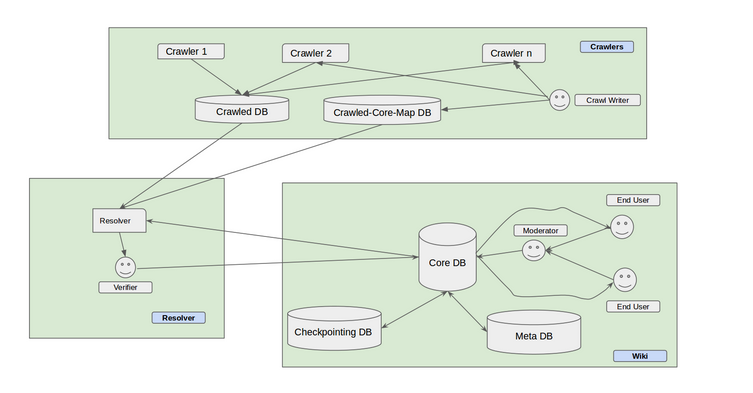
\includegraphics[scale=0.4]{sys_pipeline} 
\caption{System pipeline}
\label{fig:sys_pipeline}
\end{center}
\end{figure}
The total pipeline of the system can be seen in figure above. Overall, we have decomposed the system into 3 cohesive modules. In order of the data flow, they are - 
\begin{quotation}
Crawlers $\rightarrow$ Resolver $\rightarrow$ Wiki
\end{quotation}

\section{Crawlers}
%\lipsum[2]
This is the data acquisition module we have designed. Internally this module consists of the following components:

\subsection{\textbf{Crawler(s)}} - These are basically python scrapy/beautiful soup/selenium scripts to crawl particular websites and srape data from them. The nature of the data (i.e - data types, labels) is mentioned in the \emph{\textbf{Crawled-Core-Map}} database.

\subsection{\textbf{Crawled-Core-Map database}} - Contains the type of the data, its name(or label) to be scraped from a website. This mapping information is used by crawlers to produce output data of specific type,label. This map along with the specific crawlers are written by the developers (\emph{\textbf{Crawl-Writers}})

\subsection{\textbf{Crawled database}} - The raw output from the crawlers is written here. The schema of this database is largely dictated by the \emph{\textbf{Crawled-Core-Map}} database. The data is then read from this database into the \emph{\textbf{Resolver}} module.

\subsection{\textbf{Crawl Writers}} - They are the human components of this module. These persons are developers who write specific scripts to scrape desired websites. They are also responsible for maintaining the data schema in \emph{\textbf{Crawled-Core-Map}} database.



\section{Resolver}
%\lipsum[3]
This module works to fine tune the data scraped by the crawlers. All data collected thus far are mostly unformatted with duplicate or missing values. The function of this module is to process such data into a form suitable for the database.
Its constituents are:


\subsection{\textbf{Resolver}} - It takes the data from the Crawled database as input. The resolver can be further divided into two parts -

\begin{itemize}
\item\textbf{Cleaner} - The cleaner does the text normalization before the actual process for resolving begins. This includes out-of-format data, capitalization, missing-value issues which if not dealt with may cause the resolver to give low accuracy.
\item\textbf{Resolver/Duplicator} - Function of resolver is two-fold. Firstly, it checks any duplicate records in the incoming data (i.e. - data from the crawled database) and removes if any. Then, it resolves the entries from the crawled data with that of the core data. And outputs all possible matchings to the verifier for verification/tagging. 
\end{itemize}

\subsection{\textbf{Verifier}} The authenticity of the data should be checked before it can be inserted into the \emph{\textbf{Core Database}}.  The function of the verifier module and thus the human moderator is to tag the records outputted by the resolver module. These tagged records are the ones which are finally added to the \emph{\textbf{Core Database}}.


\section{Wiki}
This module is the web portal that is directly accessible to the end users. It consists of the interfaces that allow user to view, add, delete entities and their relationships interactively. 

\subsection{\textbf{Core Database}}
This is the main data store of the system. Care has been taken to ensure that whatever data goes in is redundant, free of noise and authenticated. \textbf{Neo4j GraphDB} \cite{Neo4j} is used in the backend for this. 

\begin{itemize}
\item\textbf{Why Graph database preferred here?}\\
Lot of brainstorming went in deciding to use Neo4j graph database. This is because a graph database stores the relations of records in the physical layer (unlike relational database) which makes faster retrieval of connections of entities without joins. And most of the analysis in social networks involves reading in the relationships/connections between entities. Hence query results can be produced faster here without any complicated joins.
\end{itemize}

\subsection{\textbf{Meta Database}} 
This contains the description of the data(format, source, type) being inserted in the database. This is especially useful when the data is authenticated against real-world information, so that every ounce of data in the core database is accounted for.
\subsection{\textbf{Checkpointing Database}}
Without a checkpoint, a Wiki is un-achievable. With every new update, a log of all changes is stored in this database. This is later used to roll back to a previous state to undo any new updates that occured. 
\subsection{\textbf{Web Server}}
Background server that hosts the web application currently has 3 major functions.
\begin{itemize}
\item\textbf{Wiki + Visualization} - The basic functionality of the web application is to provide the users with profiles and connections of organizations and personas which they can edit. The server also maintains a mechanism for checkpointing any data received.
\item\textbf{Query Engine} - To support the queries required for analysis of the network the server implements a query engine which takes queries of specific pattern and return results in tabular or visual format. This is achievable by Cypher query language which facilitates inquiring graph-like queries over Neo4j. These queries would go on the lines like: How are two entities connected? What is the shortest path between two entities? How far an influence of an entity goes over the graph? 
\item\textbf{Read API} - External applications can give GET requests to read data in json format. This aids research and analysis by end users.	
\end{itemize}
\subsection{\textbf{Others}}
Human components in the system - \emph {Users} and \emph{Moderators}. Users include the wiki-users who edit the Wiki to enter any new/updated info they have. They have to provide an evidential link for any information they commit.\\
The job of moderators is to verify records entered by users in the Wiki. They can be experts in their domain, they need to cross-verify from trusted sources.

\section{Example}
%\lipsum[2]
Here we describe how the Verifier and Resolver actually work with a working example.
\subsection{\textbf{Verifier + Resolver}}	
\begin{table}
\centering
\begin{tabular}{| c | c | c |}
\hline
{\bf Name} & {\bf Age } & {\bf Sex }\\
\hline
\end{tabular}
\caption{Sample data formats}
\label{table:1}
\end{table}


\begin{table}
\centering
\resizebox{\columnwidth}{!}{
\begin{tabular}{| c | c | c | c | c | c |}
\hline
{\bf Entity no. } & {\bf Graph label } & {\bf Graph props } & {\bf Mysql props } & {\bf Graph resolve props } & {\bf Mysql resolve props }\\
%1 & person & name,age,sex & name,age,sex & name & name \\
\hline
1 & person & name,age,sex & name,age,sex & name & name \\
\hline
\end{tabular}
}
\caption{Sample record of Crawled-Core-map database}
\label{table:2}
\end{table}

Let us say that the crawler crawls data and saves it in a format like in Table - \ref{table:1}
Also the crawler has an accompanying map-data information which looks like - \ref{table:2}\\
\emph{graph-props} column have one to one order wise mapping with \emph{mysql-props} column.\\
\emph{graph-resolve-props} column have one to one order wise mapping with \emph{mysql-resolve-props} column.\\

So, basically in the crawled data, each row represents a node with label :person and attributes (name, age, sex) in the core database.\\

\begin{enumerate}
\item Now, when a verifier logs-in a row from the \ref{table:1} is fetched, then \ref{table:2} is used to frame a query to search an entity with the name like in the row.
\item Matching nodes are suggested after the query to the verifier.
\item If verifier selects one of the propsed nodes, the resolved node is updated.
\item Else if the verifier doesn't find any matching node, a new node correspoding to the selected row is created and inserted in the core database.
\end{enumerate}

\subsection{\textbf{Wiki + Visualizations }}

\textbf{Profiles}\\

Following is a typical profile in the Wiki-

\begin{figure}[here]
\begin{center}	
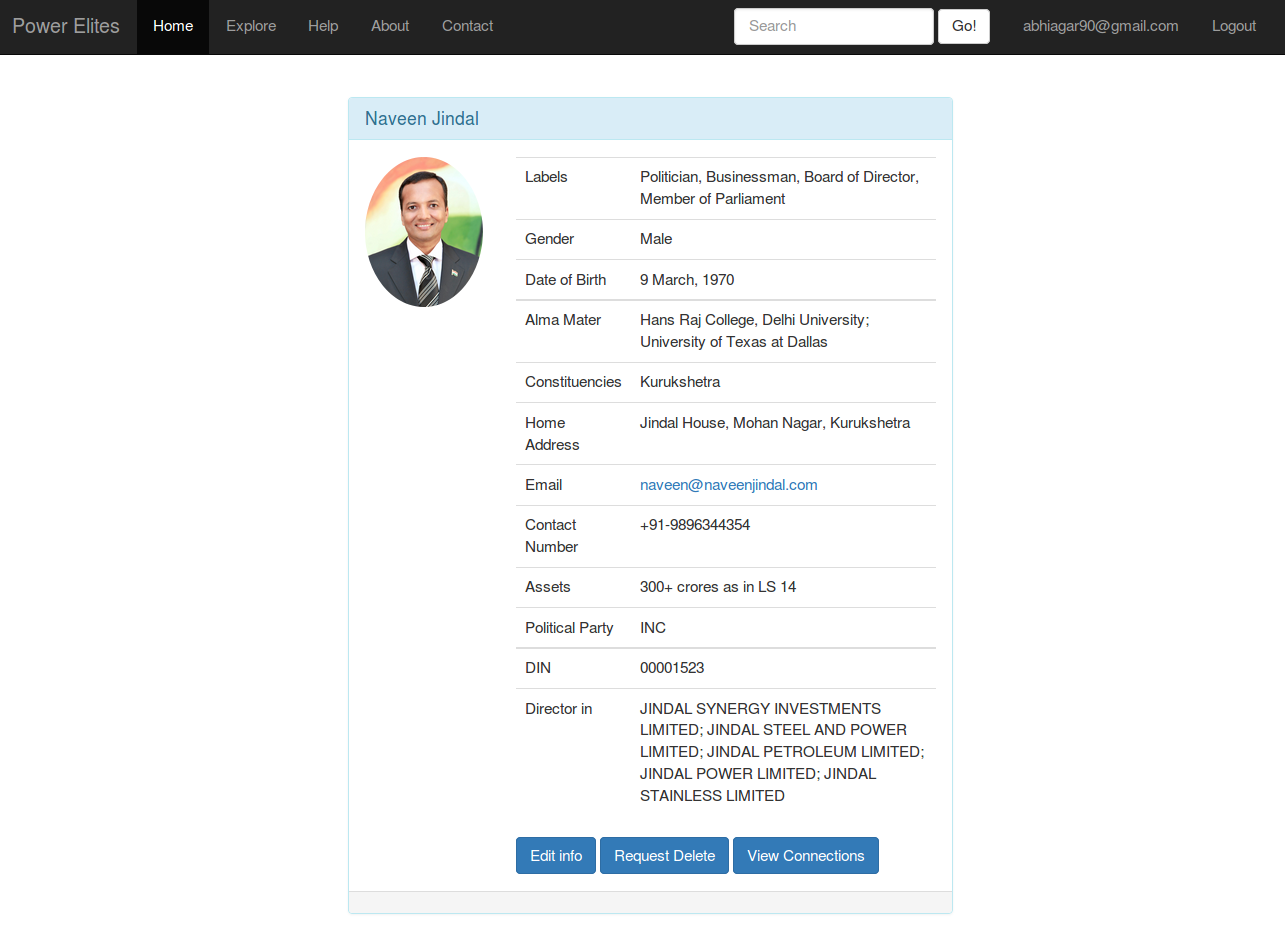
\includegraphics[width=\textwidth]{Jindal} 
\caption{Naveen Jindal Profile}
\label{fig:jindal}
\end{center}
\end{figure}

The figure above shows the Wiki page for industrialist Naveen Jindal containing information about him. It also contains interfaces for any registered user to edit as happens in a Wiki. It also allows the user to show connections of the person.\\

\textbf{Connections (Visualizations)}\\

\begin{figure}[here]
\begin{center}	
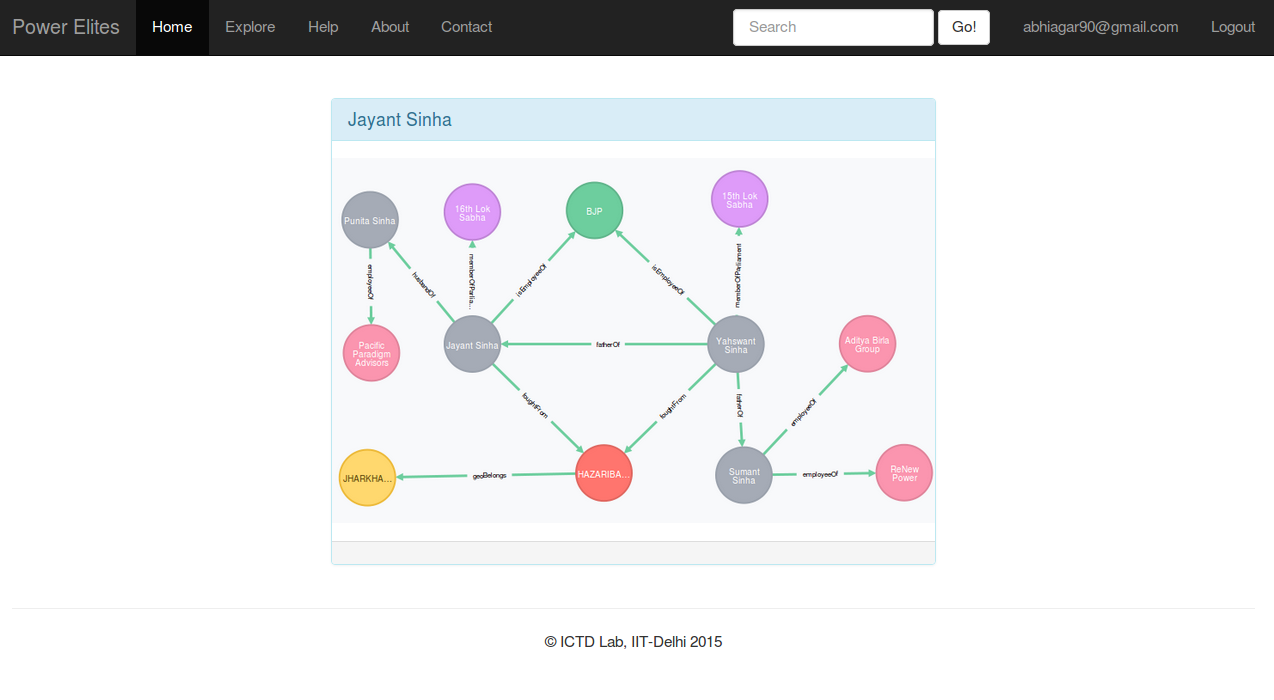
\includegraphics[width=\textwidth]{Sinha} 
\caption{Jayant Sinha Connections}
\label{fig:sinha}
\end{center}
\end{figure}
The figure above shows the connections for Minister of State for Finance Jayant Sinha. His connections include corporates firms like the \textbf{Aditya Birla Group} and \textbf{Pacific Paradigm Advisors} .

Other popular influence networks that our system shows is that of \emph{Gandhi Family and their Corporate linkups}, \emph{Jaydev Galla with his company with a large asset value}, \emph{Kamal Nath with Moser Baer}, \emph{Ravi Shankar Prasad with News 24 channel}.

\begin{figure}[here]
\begin{center}	
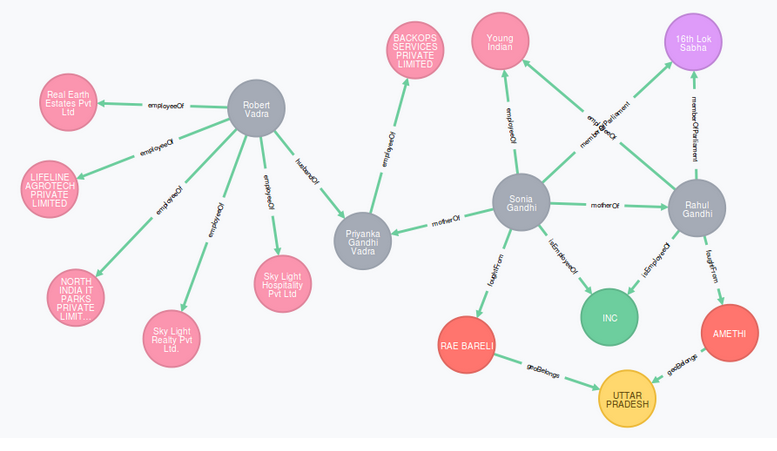
\includegraphics[scale=0.4]{Gandhi} 
\caption{Gandhi family}
\label{fig:gandhi}
\end{center}
\end{figure}

\begin{figure}[here]
\begin{center}	
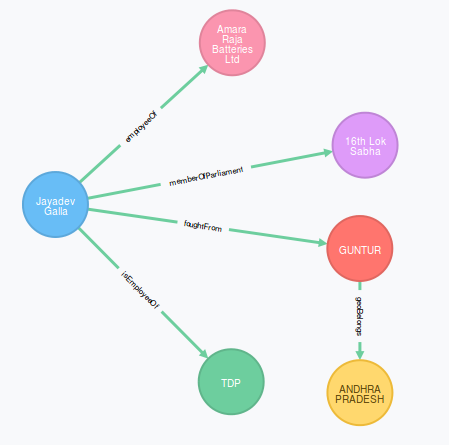
\includegraphics[scale=0.4]{Jaydev} 
\caption{Jaydev Galla Connections}
\label{fig:jaydev}
\end{center}
\end{figure}

\begin{figure}[here]
\begin{center}	
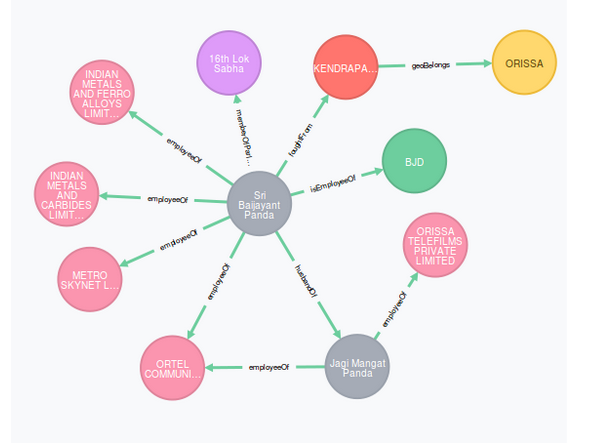
\includegraphics[scale=0.4]{Jay_Panda} 
\caption{Jay Panda Connections}
\label{fig:jaypanda}
\end{center}
\end{figure}

\begin{figure}[here]
\begin{center}	
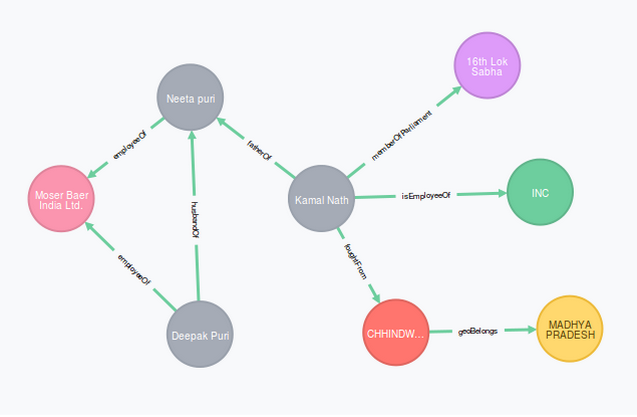
\includegraphics[scale=0.4]{Kamal_Nath} 
\caption{Kamal Nath Connections}
\label{fig:kamalnath}
\end{center}
\end{figure}

\begin{figure}[here]
\begin{center}	
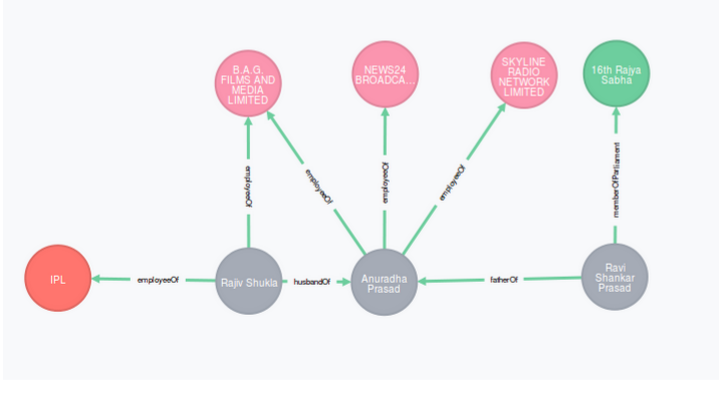
\includegraphics[scale=0.4]{Ravi_Shankar} 
\caption{Ravi Shankar Connections}
\label{fig:ravishankar}
\end{center}
\end{figure}

